\begin{frame}[fragile]{Our Problem}
  \begin{columns}[onlytextwidth, T, c]
    \begin{column}{.5\textwidth}
      initial constrainted problem:
      \newline
      \begin{equation*}
        \begin{split}
          \text{min}\ &\ \frac{1}{2} \norm{w}^2 \\
          \text{s.t.}\ &\ \forall_{i}\ y_i (x_i \cdot w + b) -1 \geq 0
        \end{split}
      \end{equation*}
    \end{column}
    \begin{column}{.5\textwidth}
        \begin{figure}
          \centering    
          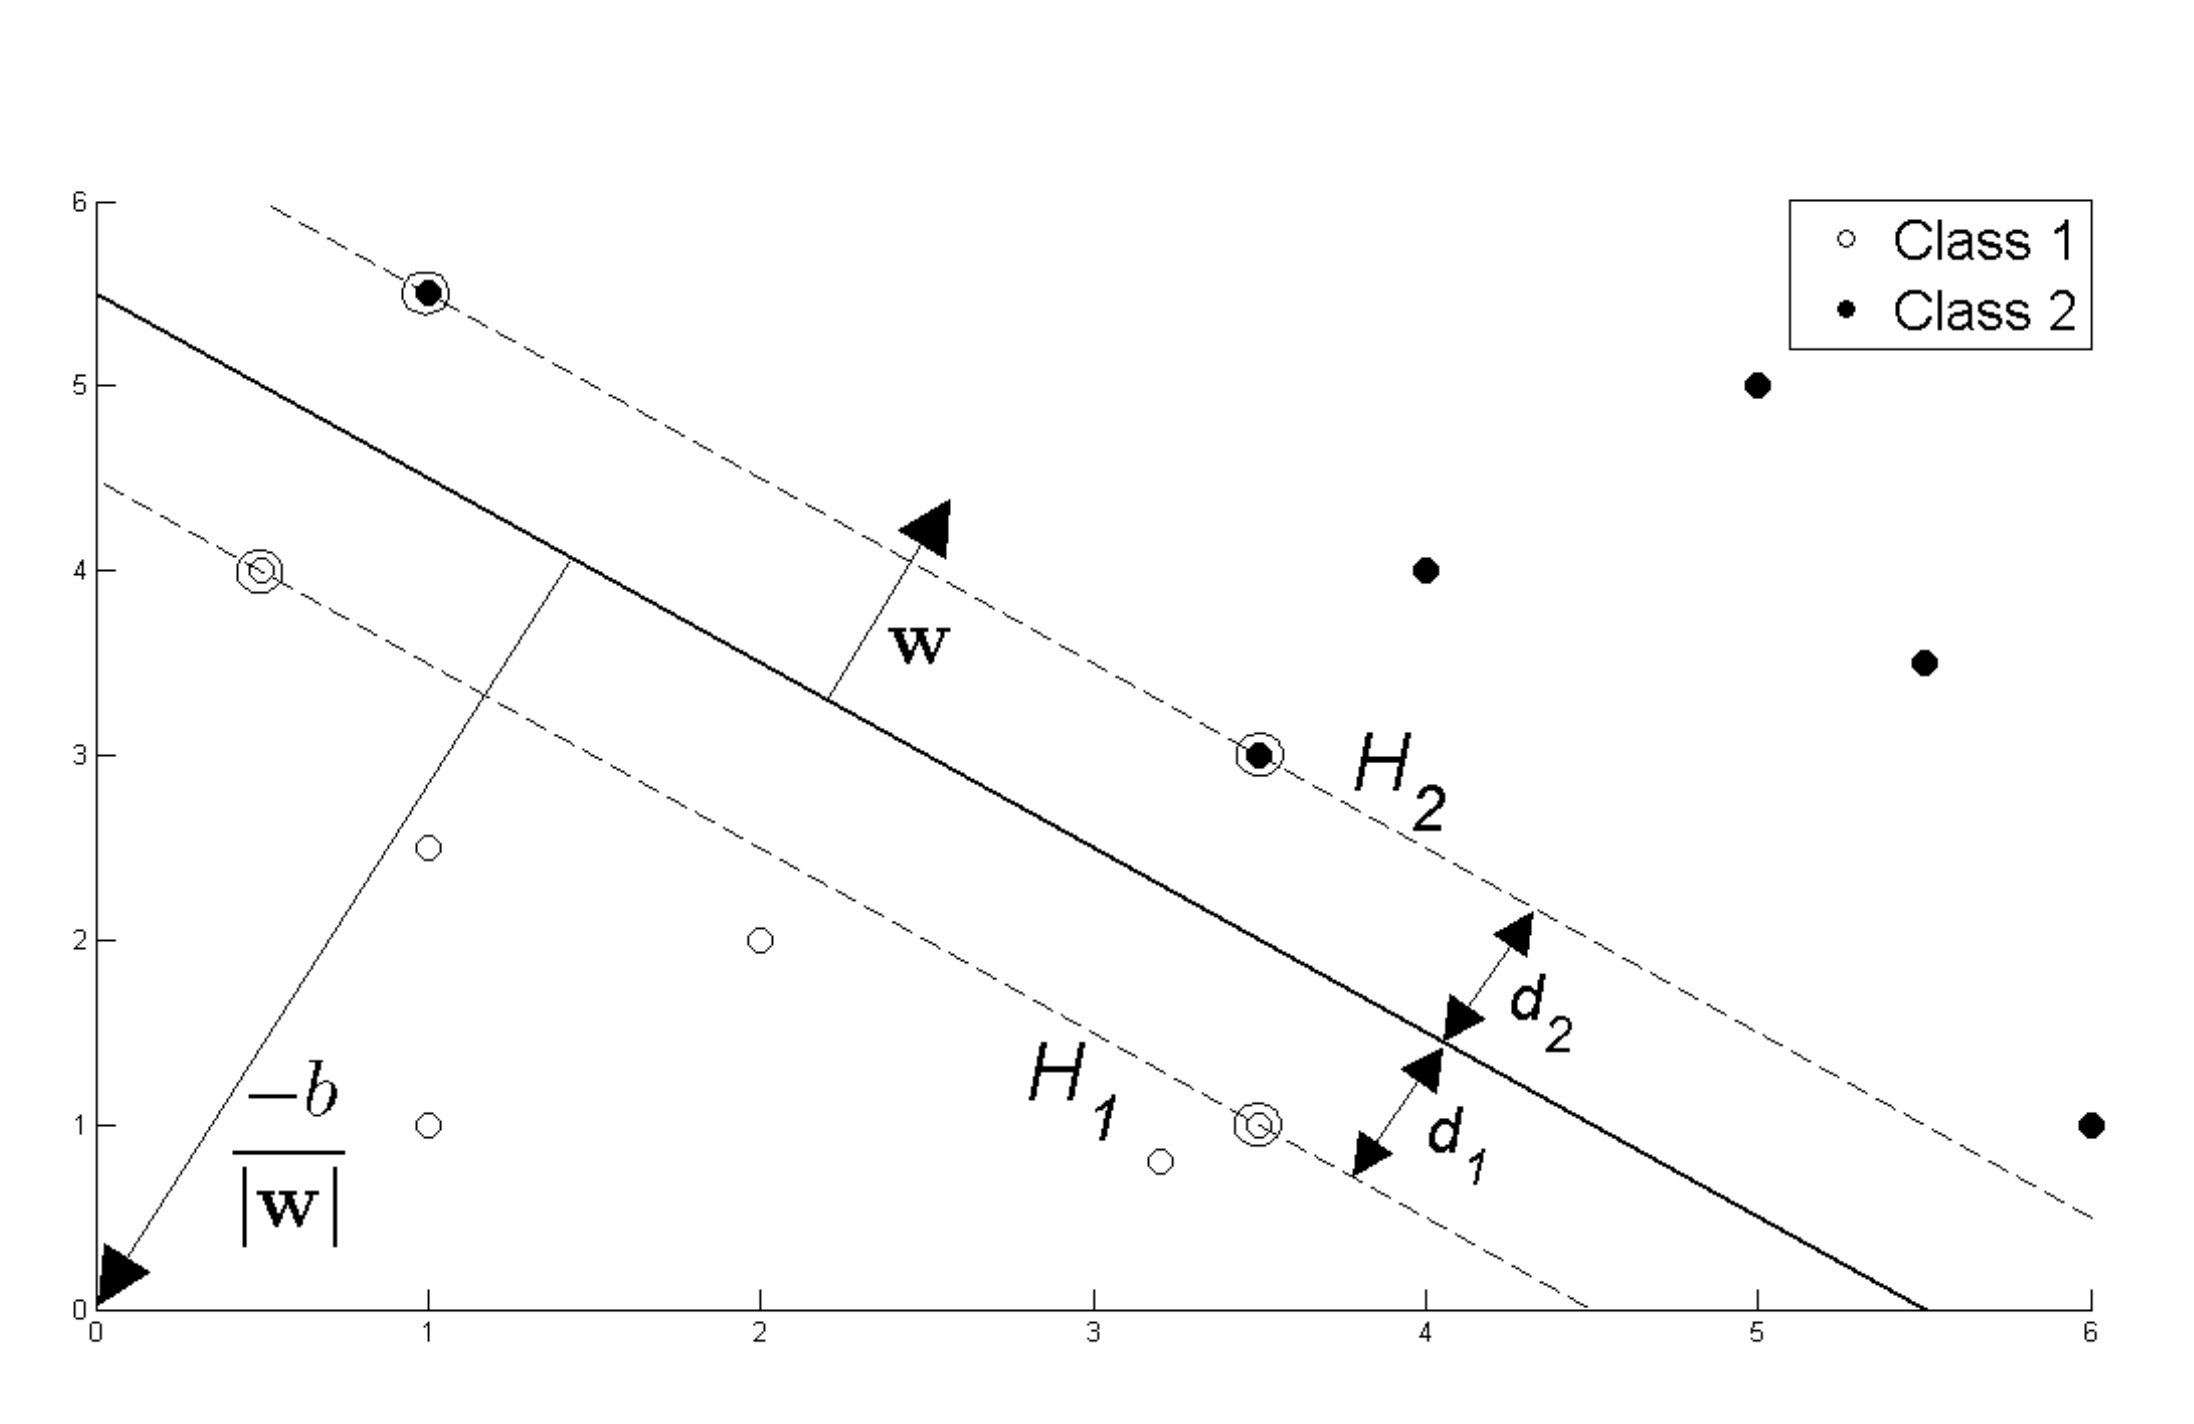
\includegraphics[width=5cm]{assets/images/s1.01.png}
        \end{figure}
    \end{column}    
  \end{columns}
  
  \vspace{.7cm}
  
  % where the hyperplane equation is $w \cdot x + b = 0$
  % and the perpendicular distance from the hyperplane to the origin is $\frac{b}{\norm{w}}$
  the points (circled) $H1$ and $H2$ that lie closest to the separating hyperplane, 
  i.e. the \textbf{Support Vectors}, can be described by
  \begin{equation*}
    \begin{split}
      x_i \cdot w + b = +1 & \hspace{.5cm} \text{for} \hspace{.5cm} H1 \\
      x_i \cdot w + b = -1 & \hspace{.5cm} \text{for} \hspace{.5cm} H2
    \end{split}
  \end{equation*}

\end{frame}


\begin{frame}[fragile]{Lagrangian Multipliers Strategy}
  we formulate our problem as:
  \newline
  \begin{equation*}
    \begin{split}
      L_P\ \equiv\ \frac{1}{2} \norm{w}^2 - \alpha [\forall_i\  y_i (x_i \cdot w + b) - 1]
    \end{split}
  \end{equation*}

  where $\alpha_i$ are the Lagrange \textbf{multipliers} such that:
  \begin{equation*}
    \forall_i\ \alpha_i\ \geq 0 
  \end{equation*}

  we want to \textbf{min} $L_P(w,b)$ and then \textbf{max} $L_P(\alpha)$.
\end{frame}


\begin{frame}[fragile]{Final Problem Formulation}
  Dual form of the primary Lagrangian problem:
  \newline
  \begin{equation*}
    \begin{split}
      \max_{\alpha}\ &\ L_D\ \equiv\ \sum_{i=1}^{L} \alpha_i - \frac{1}{2} \sum_{i,j} \alpha_i \alpha_j y_i y_j x_i \cdot x_j
      \equiv\ \sum_{i=1}^{L} \alpha_i - \frac{1}{2} \alpha^T H \alpha
    \end{split}
  \end{equation*}

  where:
  \newline
  \begin{equation*}
    H\ \equiv\ y_i y_j x_i \cdot x_j
  \end{equation*}

  subject to:
  \newline
  \begin{equation*}
    \sum_{i=1}^{L} \alpha_i y_i = 0 \hspace{.5cm} \text{and} 
    \hspace{.5cm} 
    \forall_i\ \alpha_i \geq 0 
  \end{equation*}
\end{frame}
